\section{Bayesian Probability}
\label{sec:int_bayesian_probability}

\label{subsec:int_int_bayesian_probability}

The probability theory has its roots in the $16^{th}$ century with attempts to analyse games of chance by Cardano. It is not hard to understand why games of chance are in the foundations of the probability theory. Throughout History the concept of probability has fascinated the Human being. Luck, fate were words that reflect things we feel we have no control upon and are associated with those games, and almost paradoxically we evolved in a way that we do not feel comfortable around them. 

\begin{comment}
Uncertainty raises us fear and doubt, so the games of chance provide a controlled environment in which we can make our experiments with uncertainty. Also by studying these games we seek to minimize the uncertainty associated with them.
\end{comment}


\subsection{Kolmogorov axioms}

In spite of the fact that the problem of games of chance kept attracting numerous mathematicians (with some of the most influential ones being Fermat, Pascal and Laplace), it was not until the $20^{th}$ century that the Russian mathematician Kolmogorov laid the foundations of the modern probability theory (first published in 1933) introducing three axioms\cite{sep-probability-interpret}:

\begin{enumerate}
\item The probability of an event is a non-negative real number:
\begin{equation}
 P(A)\in\mathbb{R\;}\wedge\; P(A)\geq0
\end{equation}
This number represents the likelihood of that event happening, the greater the probability the more certain is its associated outcome. 
\item The sum of probabilities of all possible outcomes in a space is always 1 ($P(\Omega)=1$). These first two axioms leave us with the corollary that probabilities are bounded:
 \begin{equation}
0\leq P(A)\leq1
\end{equation}
\item The probability of a sequence of pairwise disjoint events is the sum these events. A corollary of this axiom is:
\item Any countable sequence of mutually exclusive events satisfies:
\begin{equation}
P(A_{1}\vee A_{2} \vee ... \vee A_{n})=P(A_{1})+P(A_{2}) + ... + P(A_{n})
\end{equation}

\end{enumerate}

Another important corollary derived from the axioms is the addition law of probability:
\begin{equation}
P(A\vee B)=P(A)+P(B) - P(A\wedge B)
\end{equation}

\begin{comment}
The philosophical concept of probability has attracted some interpretations. Laplace was the first to provide a rigorous definition of probability (classical interpretation), that stated that the probability of an event could be obtained through the sum of elementary events divided by the sum of all possible events. Another approach to probabilities is the frequencist approach where the probability is considered an intrinsic part of a physical system that can be revealed through repeated probation. 

The Bayesian approach to the interpretation of probability is to consider the probability of an event the subjective degree of belief attributed by a Human. The subjective value attributed to an event in the Bayesian approach is called probability prior and it reflects a degree of belief in the uncertainty associated with the event before presenting any evidence. This prior probability could be obtained by counting, using a frequencist approach to determine probabilities. 

\end{comment}


%prooffed
\subsection{Conditional Probability}
\label{subsubsec:conditionalprobability}
When some evidence is presented we have what we can conditional probability (or posterior probability). Conditional probability  is represented as $P(A|B)$, that could be read as: the probability of A after evidence B is presented. 

The product rule is used to calculate posterior probability\ref{eq:bayesian_prababiity_product_rule}.
\begin{equation}
\label{eq:bayesian_prababiity_product_rule}
P(A|B)=\frac{P(A\wedge B)}{P(B)}
\end{equation}

%prooffed

\subsection{Joint Distribution}

When we need to deal with more than a one Boolean variable, the joint distribution is used to define events in terms of those variables. 
This distribution grows exponentially (for $n$ variables, there are $2^{n}$ combinations), with the probability space of the various variables considered. If we consider the joint probability distribution between all the variables in a given domain we call this full joint probability.
%, and the tensor product is an inherent part of the definition of the joint probability space

Assuming that have three random  variables X, Y and W representing medical inferences. X represents if a person has fever, $x$ being the answer 1 (true) or 0 (false). Y represents if a person has been in a tropical region. W stands for if a person has headaches. Their joint distribution can be considered a vector with length 8 accounting for the multiple combinations of X, Y, and W. For example $P(101)$ represents the probability of having fever and seizures without having been in a tropical region. The notation $P(xyw)$ is equivalent to $P(x,y,w)$, and to $P(X=x \vee Y=y \vee W=w)$

The joint distribution can be calculated using conditional probabilities by the chain rule\cite{Norvig2003}. Given a set of variables $x_{1},x_{2},..., x_{n}$ :
\begin{equation}
P(x_{1}, ..., x_{n})=P(x_{1}) \prod_{i=2}^{n}P(x_{i}\vert x_{i - 1}, ... , x_{1})
\end{equation}
For the last example a chain rule to calculate the joint probability would be:
\begin{equation}
\label{eq_chain_rule_example}
P(x,y,w)= P(x \vert y, w) . P(y \vert w) . P(w)  
\end{equation}

To calculate P(x) from a joint distribution we need the marginal distribution $P_{X} : x \rightarrow \sum_{w \in W} \sum_{y \in Y}P(x , y, w)$. This would require $2^{n-1}$ sums. 


\subsection{Conditional Independence}

When variables are independent they are uncorrelated and their marginal distributions are equal to their prior probability distribution\cite{Pearl2000}. For example: 
\begin{equation}
 P_{X}(x) = \sum_{w \in W} \sum_{y \in Y}P(x , y, w) = P(x) 
\end{equation}

So, two variables are independent iif \cite{feller1}\cite{Norvig2003}:

\begin{equation}
P(X\vert W) = P(X)
\end{equation}

That means if we are presented with three variables  X, Y and W that are conditional independent relatively to each other, their joint distribution would only account their probability prior probability functions, thus simplifying the chain rule (Equation \eqref{eq_chain_rule_example}):
\begin{equation}
P(x, y , w) = P(x) . P(y) . P(w)
\end{equation}

Although it isn't always possible to decouple variables and assume that they are conditionally independent, doing so is a way to counter the ``curse of dimensionality". 





\begin{comment}

\subsection{Bayes' Rule}
From $P(A|B)$ and $P(B|A)$ Thomas Bayes derived the Bayes' Law:

\begin{equation}
\label{eq_bayesrule}
P(A|B)=\frac{P(B|A).P(A)}{P(B)}
\end{equation}

The Bayesian probability is based in the Kolmogorov axioms, and can be seen as an extension of logic which allows to reason with propositions with an uncertain truth value ($P(true)=1$ and $P(false)= 0$) instead of being purely set based. 
The substitution of propositional variables for events is possible by a corollary of the "Stone's representation theorem for Boolean algebras".  \cite{VanRijsbergen2004} . This theorem was first proved by Stone (1936) and arose from a study of the spectral theory of operators on a Hilbert space.

If we consider $\Omega_{A}$ a finite set with n elements. A probability distribution on $\Omega_{A}$ is a function 
\begin{equation}
f:\Omega_{A}\rightarrow[0,1]
\end{equation}

%The set comprising all the distribution functions on $\Omega_{A}$ is denoted by $\mathcall{P}_{A}.
\subsubsection{Bayesian Inference}

The Bayes' Law is used to update the prior probability of an hypothesis ($h$), as evidence ($E$), is presented in a process named Bayesian Inference as in the equation \eqref{eq_bayesrule_i}.

\begin{equation}
\label{eq_bayesrule_i}
P(h|E)=\frac{P(E|h).P(h)}{P(E)}
\end{equation}

 If we have a set of hypothesis $h_{1}, h_{2}, ..., h_{n}$ to explain some evidence (symptoms of a disease, for example), we would be interested in the most probable hypothesis a posteriori (after presenting the evidence), $h_{MAP}$.

\begin{equation}
\label{eq_bayesrule_ii}
h_{MAP}= argmax_{h_{i}}\frac{P(E|h_{i}).P(h_{i})}{P(E)}
\end{equation}

As we are maximizing, we can dispose of the common denominator.

\begin{equation}
\label{eq_bayesrule_iii}
h_{MAP}= argmax_{h_{i}}P(E|h_{i}).P(h_{i})
\end{equation}

This allows for the definition of the scores 

\begin{equation}
P(E|h_{MAP}).P(h_{MAP}) 
\end{equation}

and

\begin{equation}
 P(E|\lnot h_{MAP}).P(\lnot h_{MAP})
\end{equation} 

By the law of total probability

\begin{equation}
\label{eq_law_total_probability}
1= P(h|E)+P(\lnot h|E)
\end{equation}

we can attain $P(h|E)$ and $P(\lnot h|E)$ by normalization as

\begin{equation}
\label{eq_bayesrule_alpha}
1 = \alpha < P(h|E) ; P(\lnot h|E)>
\end{equation}

This leaves us with a way to calculate $P(h|E)$ :

\begin{equation}
\label{eq_bayesrule_iiiii}
P(h|E)= \frac{P(E|h).P(h)}{P(E|h).P(h) + P(E|\lnot h).P(\lnot h)}
\end{equation}

\subsection{Joint Distribution}

When we need to deal with more than a one variable, the joint distribution is used to define events in terms of those variables. 
This distribution grows exponentially (for $n$ variables, there are $2^{n}$ combinations), with the probability space of the various variables considered. If we consider the joint probability distribution between all the variables in a given domain we call this full joint probability.
%, and the tensor product is an inherent part of the definition of the joint probability space

Assuming that have three random  variables X, Y and W representing medical inferences. X represents if a person has fever, $x$ being the answer 1 (true) or 0 (false). Y represents if a person has been in a tropical region. W stands for if a person has headaches. Their joint distribution can be considered a vector with length 8 accounting for the multiple combinations of X, Y, and W. For example P(101) represents the probability of having fever and seizures without having been in a tropical region.

The joint distribution can be calculated using conditional probabilities by the chain rule. Given a set of variables $x_{1},x_{2},..., x_{n}$ :
\begin{equation}
P(\cap_{i=1}^{n}x_{i})=\prod_{i=1}^{n}P(x_{i}\vert\cap_{j=1}^{i-1}x_{j})
\end{equation}
For the last example a chain rule to calculate the joint probability would be:
\begin{equation}
\label{eq_chain_rule_example}
P(x,y,w)= P(x \vert y, w) . P(y \vert w) . P(w)  
\end{equation}

To calculate P(x) from a joint distribution we need the marginal distribution $P_{X} : x \rightarrow \sum_{w \in W} \sum_{y \in Y}P(x , y, w)$. This would require $2^{n-1}$ sums. 


\subsection{Conditional Independence}

When variables are independent they are uncorrelated and their marginal distributions are equal to the prior probability distribution which is attributed to each variable in cause\cite{Pearl2000}. For example: 
\begin{equation}
 P_{X}(x) = \sum_{w \in W} \sum_{y \in Y}P(x , y, w) = P(x) 
\end{equation}

So, two variables are independent iif \cite{feller1}\cite{Norvig2003}:

\begin{equation}
P(X\vert W) = P(X)
\end{equation}

That means if we are presented with three variables  X, Y and W that are conditional independent relatively to each other, their joint distribution would only account their probability prior probability functions, thus simplifying the chain rule (Equation \eqref{eq_chain_rule_example}):
\begin{equation}
P(x, y , w) = P(x) . P(y) . P(w)
\end{equation}

Although it isn't always possible to decouple variables and assume that they are conditionally independent, doing so is a way to counter the ``curse of dimensionality". 
\end{comment}

\subsection{Markov Chains}
\label{subsub:MarkovChains}
Markov Chains define a system in terms of states and the probabilistic transitions from one state to another. 

\begin{figure}[h]
\centering 
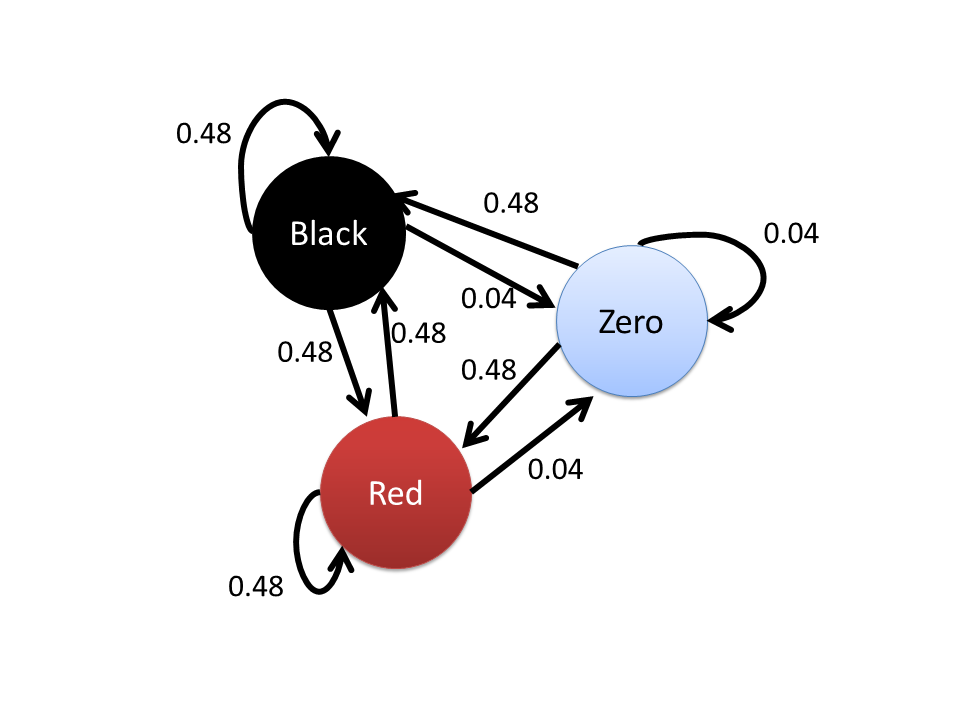
\includegraphics[scale=0.30]{Figures/RouletteMC.png}
\caption{Markov Chain of a perspective on a roulette.}
\label{fig:roulette}
\end{figure}

In 1913, at Monte Carlo Casino (Monaco), black came up twenty-six times in succession in roulette. Knowing that the probability of the ball landing on a red or on a black house is approximately $0.48$ (the zero is a neutral house), many a gambler lost enormous sums while betting red as the they believed that the roulette was ripe with red, given the history. Players didn't want to believe that this and insisted that the roulette was biased; this became known as the Gamblers fallacy.


In the Markov Chain represented on Figure \ref{fig:roulette}, we can see that in the state black the probability of transitioning to red is the same as to stay on the state black.

Given a system represented by the states $\{ x_{0}, x_{1}, ..., x_{i}, ..., x_{n}\}$, and considering $ p_{ij}$ the probability of being in the state $j$ and transitioning to the state $i$, the mixed state vector \ref{eq:prob_mixed_vector}, which represents the probabilities of the system in the that $i$ to transition to the other states. .

\begin{equation}
\label{eq:prob_mixed_vector}
\overrightarrow{x_{i}}  = \{ p_{0i}x_{0} , p_{1i}x_{1}, ... ,  p_{ii}x_{i}, ..., p_{ni}x_{n} \}
\end{equation}


The law of total probability is verified as $\sum_{j=0}^{n}p_{ji}=1$, by specifying the every transition we get a stochastic matrix $P$, named the Markov matrix.

To illustrate how to construct a Markov Chain we will pick up on the example of Figure \ref{fig:roulette}. 

In this simplification of the Roulette we have $3$ states:
\begin{itemize}
\item Black (B);
\item Red (R);
\item Zero (0).
\end{itemize}

We indifferently assign an index to each state, in order to construct the mixed state vector as in \ref{eq:prob_mixed_vector}. Having the mixed state vectors defined the next step is to use them to create the stochastic matrix that has specified every transition \ref{eq:prob_markov_matrix}.

\begin{equation}
\label{eq:prob_markov_matrix}
R=\left[\begin{array}{ccc}
p_{BB} & p_{BR} & p_{B0}\\
p_{RB} & p_{RR} & p_{R0}\\
p_{0B} & p_{0R} & p_{00}
\end{array}\right] = \left[\begin{array}{ccc}
0.48 & 0.48 & 0.04\\
0.48 & 0.48 & 0.04\\
0.48 & 0.48 & 0.04
\end{array}\right]
\end{equation}





\begin{comment}

\subsubsection{Hidden Markov Models}
\ac{HMM} are a temporal statistical tool, known as Markov Model, which allows representing systems where we have a hidden layer and an output layer, that depends on the hidden layer\cite{eemcs5901}\cite{Norvig2003}. An example of a simple Markov Model could be a Markov Chain. However Markov Chains do not have hidden layers because the state of the system is completely visible to the observer; in the roulette example (Figure \ref{fig:roulette}), we know at each moment which if we have a red house. 

In \ac{HMM}, the hidden states are not directly visible, only the output is visible\cite{citeulike:405907}. So, in order to predict the current state of the hidden layer we take into account past outputs. 

\end{comment}






